\chapter{Design and Implementation} \label{methode}
In this chapter, we will present our implementation of the sparse matrix-vector multiplication (SpMV) over boolean semiring, how we implemented with HLS and how we connected the IP-cores in the FPGA.

\section{IP-core}
For this project, we have implemented an IP-core with Vivado HLS. The IP-core applies a modified version of SpMV over an adjacency matrix and a set of vertices known as seed nodes. We will give a brief introduction to HLS programming and how to customize the algorithm for HLS.

\subsection{High Level Implementation}
Our implementation of the SpMV is done in HLS. The algorithm takes in an adjacency matrix and a set of seed nodes as input and outputs a result vector showing which vertices were activated. The algorithm stops when all the vertices have been activated or it is unable to find any new candidates. Unlike normal SpMV, where each iteration will activate all their neighbours, an ICM is dependent on random number generator (RNG) and a global or local probability. For this project a global probability of 5\% was used, i.e. each vertex had a 5\% chance of being activated. If $v_1$ was not activated by $V_r$ on the first iteration, $V_r$ can not reactivate $v_1$ on the next iteration. To prevent a reactivation, as mentioned above, a frontier vector will be sent in instead of the result from the previous iteration. 

A vector is a list of vertices. The frontier vector is generated by comparing the result from current iteration with a list of activated vertices. The vertices that are in the frontier vector are the vertices that were not activated in the previous iteration but were activated in the current iteration. 

Our algorithm applies SpMV over the matrix and the frontier. For each iteration, each element in a row of the matrix is applied an AND (\&\&) operation with the corresponding element in the frontier vector. The results from these operations will be ORed ($\|$) together, which gives the result for the row.:
\begin{algorithm}
\begin{algorithmic}[2]
\State{(martix\_row[0] \&\& frontier[0])$\|$(matrix\_row[1] \&\& frontier[1])$\| \ldots$\\
(matrix\_row[n] \&\& frontier[n])$=$result[row]}
\end{algorithmic}
\end{algorithm}


Unlike the breadth first search on boolean semiring, each vertex will have a chance to not be activated (set as '1'), even if matrix\_row[x] and frontier[x] = 1. This resulted in that for each \&\&- operation, we need to \&\& another \textit{coin toss}, which determined if the activation takes place. The coin-toss is determined by the RNG and the global probability. 

The algorithm will continue until either all of the vertices are activated, or no more vertices can be activated. This is solved with a function dist\_gen, that stops the algorithm when either no more vertices are activated in frontier vector, or all the vertices in the result vector are activated. 

In the high-level implementation, the implementation of the algorithm was done on two levels. The top level was the \textit{TopLevelWrapper}. The TopLevelWrapper was set as the main function in our HLS implementation. The function takes in the address of the location of the matrix, the address of the result, and the address to the frontier. Since we are working with ICM, a global probability, a random seed as the initial state for the LFSR is also set as input. The  TopLevelWrapper stores the useful data in a local buffer, where it is sent to the datapath function. The datapath function is a sparse matrix-vector multiplication. 

\subsection{Seed Selection}
Seed selection that was implemented, was the greedy seed selection. Our IP-core performed ICM with an input of a set of vertices as seed nodes. The greedy algorithm was implemented on PS, and continuously sends new sets of seed nodes to the IP-core much like the \ref{fig:overviewe}. 


\begin{figure}[!]
\includegraphics[scale=0.3]{Figures/Overview_of_system}
\caption{Overview of out implementation}
    \label{fig:overviewe}
\end{figure}


The address to the matrix, result, frontier, and the random seed and global probability is all mapped as AXI4-Lite while the matrix, frontier and the result are memory mapped. This allows us to send in the address of the memory location where the variables are stored and apply our algorithm. 
 
Since ICM is dependent on a random function, we ran each set of seed nodes 50 times to find the average runtime and coverage to find the most optimal set of vertices.

\section{Linear-Feedback Shift Register}
The LFSR is a commonly used pseudorandom number generator(pRNG)\citep{murase1992linear}. Different sized LFRS can generate a wider range of pseudorandom numbers. LFSR generates a pseudorandom number based on the previous pseudorandom number it generated. The LFSR implemented for this project is a 16-bit shift register, that can generate a pseudorandom number in the range from 0-$2^{16}(65536)$. To generate the new number, the bits from positions 16,14,13 and 11, is XORed. I.e. (((16 XOR 14) XOR 13 ) XOR 11) = new bit. The new bit is pushed into bit position 1 and the entire registers shifts towards right 1 bit. 
This allows the IP-core to generate a pseudorandom number based on an initial seed input. From Figure: \ref{fig:LFSR} we can see that to continuously generate pseudorandom numbers the output from the LFSR is used as the next iterations seed. 

\begin{figure} 
\includegraphics[scale=0.5]{Figures/LFSR}
\caption{16-bit Linear-Feedback Shift Register}
    \label{fig:LFSR}
\end{figure}




\section{Design flow of HLS}

\begin{wrapfigure}{r}{0.5\textwidth}
\includegraphics[scale=0.5]{Figures/HLSworkflow}
\caption{Diagram of HLS wokflow}
    \label{fig:hlsworkflow}
\end{wrapfigure}


For this project, Xilinx Vivado HLS 2016.1 was used. The usual workflow in designing with Vivado HLS is as follow. 

\begin{enumerate}
\item Define your function/algorithm.
\item Simulate as compile code. 
\item Synthesise.
\item Co-simulate.
\end{enumerate}


There are some steps that Vivado HLS requires before the project can start. In the beginning, Vivado HLS would require the designer to specify which function is the top level of the implementation. That top function would determine which port the IP core would have and what type of AXI4 protocol to implement. Vivado HLS also enables the user to specify to which platform this implementation is for.


The first step in designing with Vivado HLS is to define the algorithm that will be synthesised. E.g. for this report, it is the matrix-vector multiplication. After identifying different requirements and dependencies, the algorithm is implemented in C with Vivado HLS. Vivado HLS has some limitation regarding the high-level implementations:
\begin{itemize}
\item No dynamic memory (Need to be static), Vivado HLS does not support malloc, free, new or delete. 
\item NO STD, FILE-IO, etc., (no system calls). 
\item avoid recursive functions. 
\end{itemize}

The next step is to \textit{run C simulation}. This will verify that the C implementation is correct, by running the test in the testbench. The test in the testbench is created by the designer. After verifying that the implementation is correct, next step is to synthesise the implementation. Vivado HLS will then generate the appropriate Verilog or VHDL, depending on the designer choice. The finished generated solution is then reviewed by reading the Vivado synthesis report. The report containing crucial information regarding the generated solution. There we can find the performance estimates of the generated core, the utilization estimates, and the interface to the generated core. After all, this is done, Vivado offers a \textit{run C/RTL Cosimulation}. Vivado will then run both the C simulation and testbench, and the same testbench on a simulated version of the implemented core. This function allows the designer to verify that the generated core have the same behaviour as the simulated C implementation.

After Cosimulation is done, the IP-core is ready for export. \textit{Export RTL} generates the necessary RTL files and exports the IP core. The exported IP-core can then be found in the project folder and is ready to be uploaded to the FPGA. 

The input and output port of the IP core is determined by the variables that the top function requires. variables that are read from will automatically be set as input, while variable that are only written to, will be set as output. In order for the core to understand what is mutable, the output is often set as a pointer (For C code). VIVADO HLS generates control signals cl automatically. 

\section{Network and graph generator}

For this project, we choose to implement a R-mat generator as mentioned in Chapter: \ref{rmat} and  \cite{Rmat2004}. The generator is implemented in \textit{Python} \cite{PYTHON} with \textit{numpy}. The generator generates adjacency matrix with $2^k$ vertices, where \textit{k} is known as the scale of the sparse matrix. The total amount of edges the graph contains is set as $total\_amount\_of\_edge = k \times\ edge\_factor $. The edge factor is the ratio between the graph's edge count and ins vertex count\cite{graph500}.



\section{How is it connected}
As shown in Figure \ref{fig:vivadoImple}, out IP-core is the \textit{TopLevelWrapper}, and the PS is the Zynq processing system. The AXI interconnect serves as a interconnect between our IP-core and the PS.

\begin{figure}[!ht]
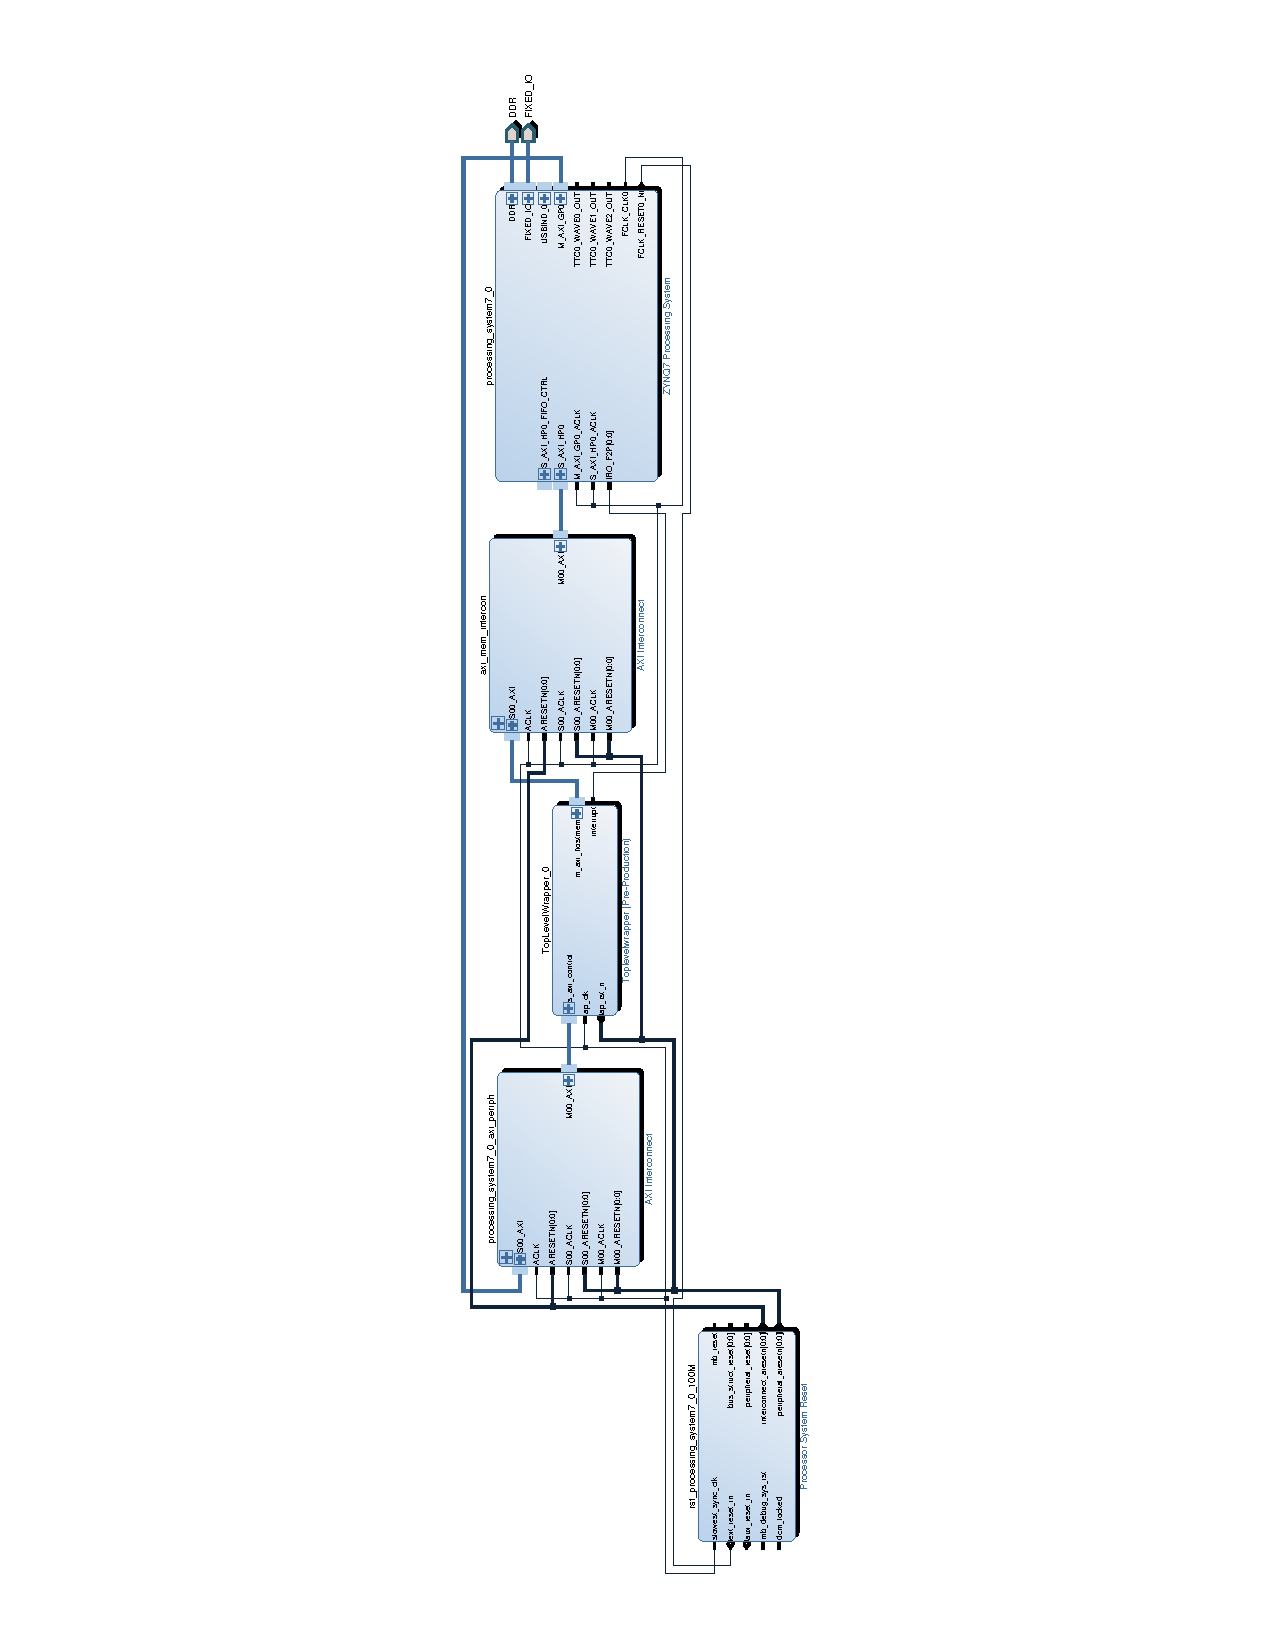
\includegraphics[scale=0.7]{Figures/design_1}
\caption{Our IP-core and how it is connected.}
\label{fig:vivadoImple}
\end{figure}



Our core is memory mapped and we use the bus interface AXI4-Lite for communication. The core includes a DMA-component, which the HLS would initiate for us. This allows us to utilize the High-performance slave interface on our PS.


\section{Xilinx SDK}
In Xilinx vivado, a Xilinx Software Development Kit was provided. In the SDK, the IP-core was initiated and control signals were set. For our experiment, the seed selection were implemented in Xilinx SDK.
%Snakk litt om hvordan din seed search er implementert via xilinx sdk%



\section{Optimization}
The function matrix\_vector\_multiplication() performs a single matrix-vector multiplication. From the pseudocode, we can see that there is  room for parallelization of the SpMV. The outer for loop from the pseudocode can be parallelized since the for loop is not dependent on the variables from the inner for-loop. 

Another possible parallelization is during the simulation, after the SpMV, the frontier vector needs to be calculated. And a converged() function is called in the end to determine if the simulation is finished. The frontier calculation and converged can be run in parallel. 

include the different directives, PIPLINE, LOOP UNROLL and DEPENDENCE. Directives are predefined optimization that HLS provides, by incorporate them in the high-level implementation, HLS would apply specific optimization. For our implementation, the following directive was added.

\begin{itemize}
\item \textbf{PIPELINE} Allows the implementation to utilize concurrent execution of operations \citep{optiDirect}. This allows loops and functions to execute in parallel. 
\item \textbf{UNROLL} generates multiple independent operations instead of sequential operation such as for-loops.\citep{optiDirect}
\item \textbf{DEPENDENCE} Provides additional information in regarding loop-carry dependency. Allows loops too be pipelined.\citep{optiDirect}
\end{itemize}


\section{Potential improvement}:
For the second option, where the RNG core is not implemented into the IP CORE, we would have to have the random number set as AXI4 stream from the buffer, since we would need to call a stream of random numbers from the core.


\section{Global vs local probability}
For this project, a global activation chance was implemented, giving each vertex the same probability to be activated. An interesting model would be there is a personal probability of activation. Each vertex might have unique activation chance. Our implementation. 
